The Behavioral and Social Sciences Laboratory provides powerful and efficient infrastructure for conducting research in the behavioral and social sciences. The Jacobs Center operates the laboratory together with the School of Humanities and Social Sciences. With over 1200 m$^{2}$ of research space, it is Europe's largest laboratory of its kind. 
\\
The laboratory forms an essential base for the research activities of the Center:
Its measurement sets for electrodermal and cardiovascular activity, eye-tracking equipment, and ergospirometry allow the examination of brain functions and age-related changes in physical and mental performance. Group and single rooms equipped with one-way mirrors, cameras, and presentation facilities allow for conducting interviews, behavior video observation, and telephone surveys; these tools are important for our researchers exploring decision-making and learning behavior. Altogether, 77 trial areas can be used, including a senso-lab (to test touch perception), motor-lab (to test fine motor skills), computer-lab (to test intelligence) and human performance lab (to test brain plasticity). 

\begin{figure}[htbp]
	\begin{center}
		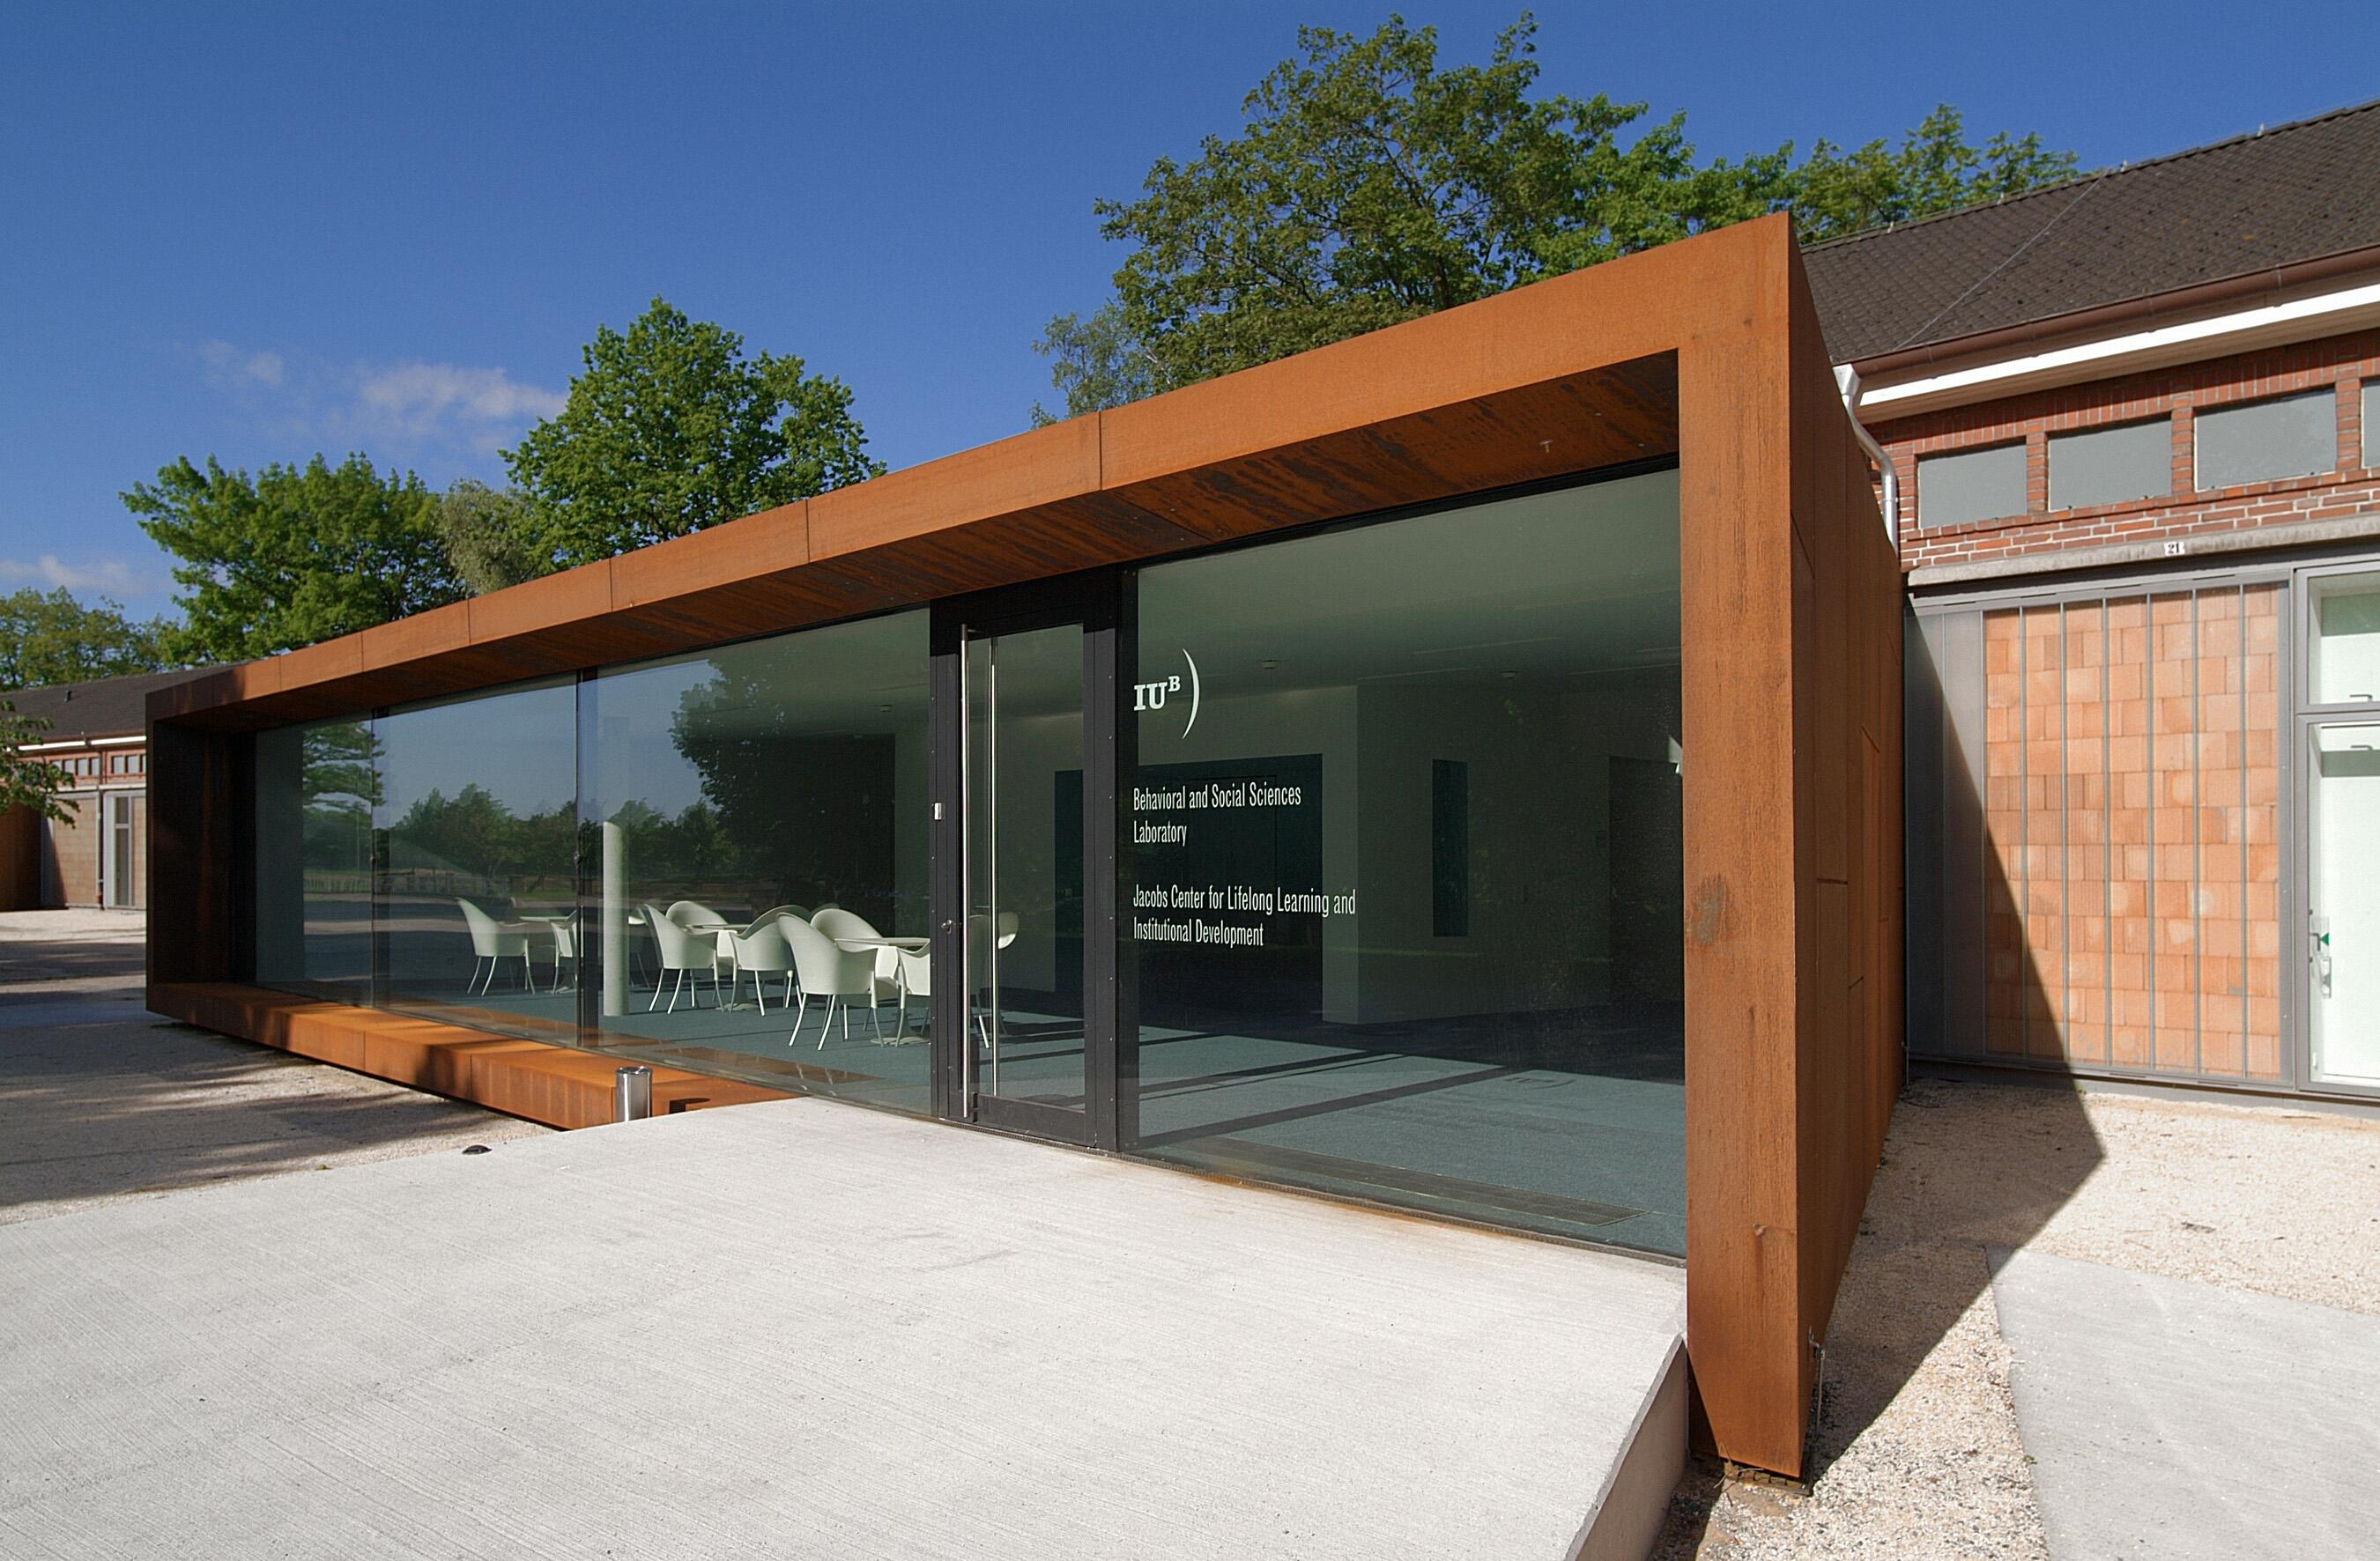
\includegraphics[width=0.5\textwidth,height=5cm]{E:/download/LateX/photo2.jpg}
	\end{center}
\end{figure}

